\chapter{Memory formation in Alzheimer's Disease}
\section{Introduction}

\section{Material and Methods}\todo{edit methods}

\subsection{Animals and vectors}
All animals were housed in groups of 4 or 5, with a 12-hour light/dark cycle. Food and water are provided \textit{ad libitum} to all animals. Experiments were performed during the light phase of the circadian cycle. Mice were at least 8 weeks old at the beginning of all experiments. All experiments were in accordance to the Hospital for Sick Children Animal Care and Use Committee.

\subsubsection{TgCRND8 mice}
TgCRND8 mice were developed at the Center of Research for Neurodegenerative Diseases (CRND) and carry a human APP695 transgene with the Swedish (K670N-M671L) and Indiana (V717F) FAD mutations under the regulation of the Syrian hamster prion promoter \citep{chishti01}. TgCRND8 was back-crossed with C57BL/6, \gls{tg} and \gls{wt} littermates of F1 generation were used in the experiments.


\subsubsection{GP5.17 mice}
GP5.17 mice transgenically express the flourescence calcium indicator GCaMP6f under the Thy1 promoter \citep{dana14}. TgCRND8 was crossed with GP5.17. Animals that that are GCaMP6f\textsuperscript{+} and \gls{app}\textsuperscript{-}, or GCaMP6f\textsuperscript{+} and \gls{app}\textsuperscript{+} are used in the experiments. 

\subsubsection{Viral vectors}
In the TgCRND8 mice, GCaMP6f expression is delivered through \gls{aav}. GCaMP6f expression is controlled by \gls{hsyn} promoter. AAV--DJ--syn--GCaMP6f virus was purchased from Stanford University Gene and Viral Vector Core. The virus is used undiluted. 

\subsubsection{\tglu peptide}
To deliever \glu construct (YKEGYNVYG) to target, we attached it to the protein transduction domain of the \gls{hiv} \textit{tat} gene (TAT peptide). The TAT peptide is able to transport across cell membrane and \gls{bbb} through an unknown mechanism \todo{cite TAT}. The \tglu was synthesized from the sequence YGRKKRRQRRRYKEGYNVYG and desolved in saline. 


\subsection{Viral Infusion}

Each animal received \gls{ip} injection of atropine (\SI{0.1}{\mg\per\kg}) and chlorohydrate (\SI{400}{\mg\per\kg}) before being secured on a stereotaxic frame. An incision was made on the scalp and the skin was pulled to the side to reveal the skull. Holes were drilled above \gls{la} on the skull for micropipette injection. Virus was loaded into a glass micropipette and gradually lowered to target coordinate. \SI{1.5}{\ul} of virus were injected on each side at a rate of \SI{0.12}{\ul\per\min}, aiming at \gls{la} (\gls{a/p} \SI{-1.4}{\mm}, \gls{m/l} $\pm$\SI{3.5}{\mm}, \gls{d/v} \SI{5.0}{\mm} from Bregma). The micropipette was left in the brain for an extra \SI{10}{\min} before slowly retracted. The incision was sutured and treated with antibiotics. Each animal then received subcutaneous injection of analgesic (ketoprofen, \SI{5}{\mg\per\kg}) before returned to a partially heated clean cage for recovery.

\subsection{Histology}
Placement of implants and extent of viral infections was determined by \gls{gfp} expression. After all experiments, animals were transcardially perfused with first \gls{pbs} then 4\% \gls{pfa}. The brains were disected and kept in 4\% \gls{pfa} overnight, and washed with \gls{pbs}. The brains were then sliced coronally on a vibrotome (\todo{vibrotome info}) to \SI{50}{\um} thickness. Slices containing \gls{la} were then mounted on gelatin-coated glass slices with a hardening mounting media (Permaflour\todo{permaflour info}) and assessed under an epi-flourescence microscope(Nikon\todo{Nikon info}).

\subsection{Contextual fear conditioning}
Fear conditioning chambers (\SI{31 x 24 x 21}{\cm}; MED Associates, St. Albans, VT), consisted of 2 stainless steel and 2 clear acrylic walls, with a stainless steel shock-grid floor (bars \SI{3.2}{\mm} diameter, spaced \SI{7.9}{\mm} apart). A plastic drop-pan containing a 70\% ethanol solution was placed below the grid floor. A fan provided low-level white- noise during training and testing in the context. Behavior was monitored by overhead cameras, which digitized video images at \SI{15}{\Hz}. 

Animals underwent contextual fear conditioning three weeks after mini-microscope baseplate implantation. One hour before training, animals received either TAT-GluA2 peptide (i.p., \SI{15}{\mmol\per\kg}) or vehicle injection. A mini-microscope is attached to the animal to record calcium activities during both training and testing of contextual fear conditioning. During training, animals were confined in the chamber for \SI{5}{\minute}. A footshock of \SI{0.5}{\mA} was delivered at \SI{4}{\minute} time point. During testing session \SI{24}{\hour} later, animals were placed back in the training environment for \SI{10}{\minute}. 

\subsection{Animal tracing}
\todo{Animal tracing method}
Videos of animal behaviours were encoded as grey-scale images. Due to a dark background, overlaying mini-microscope wire and commutators and changing shadows, no simple feature is able to reliably identify the animal from the background. Instead, we used multiple features, calculate the distribution of the features in tracked animals, and use all the features together to estimate the position of the animal for each frame. During model fitting, distribution of every feature was estimated with a gaussian kernel \todo{kernel size}.

\subsubsection{Features}

\paragraph{Pixel intensity.} Intensity of pixel at animal's position. This feature tries to capture the animal's fur colour.

\paragraph{Normed pixel intensity.} Pixel intensity of animal's position, when the frame is normalized to zero mean and unit standard deviation. This feature tries to capture animal's fur colour with minor variations in illumination.

\paragraph{Forground pixel intensity.} Pixel intensity differenece between foreground and background images at the animal's position. The background image of the environment was generated by taking the mean pixel density across time. This feature tries to separate animals to any pixels with similar colour in the background.

\paragraph{Difference to low pass intensity.} Pixel intensity difference between foreground image and low-pass filtered foreground image (\todo{window size}) at animals position. This feature tries to capture the fact that the animal's colour is close to uniform, therefore eliminates noise pixels with similar colour.

\paragraph{Speed.} Distance between animal's positions in two consecutive frames. 

\paragraph{Change in intensity.} Difference of pixel intensity at animal's positions in two consecutive frames. This feature captures the fact that animal's colour is relative consistent between frames.

\paragraph{Chaneg in intensity (blurred).} Similar to change in intensity, but using gaussian blurred images to remove effect of random noise.

\paragraph{Magnitude of accelaration.} Magnitude of accelaration vector, which calculated as the vector difference of two consecutive velocity calculations. 

\paragraph{Segmentation area.} Edges in the frame is detected (Canny, \todo{threshold size}). The edges are then morphologically closed (\todo{iterations}) to remove sporatic edges. The area enclosing the position of the animal is then calculated. This feature tries to capture the size of the animal.


\subsubsection{Tracking}
\todo{particle filter}

For a single pixel, we calculate its score as the summation of likelihood for all the features\todo{formula}. The pixel with the highest score is the most likely position of the animal. However, calculating score for every pixel is computationally intensive. Instead, we took advantage of particle filters to estimate the distribution of score over pixels. \todo{cite particle filters, formula, detailed description}.

While improvement can still be made to this method, with the current implementation the algorithm is able to correctly track animals with minimal human intervention. \todo{ref code}


\subsection{Analysis}

\subsubsection{Cell activity}

All traces were normalized to have zero median and unit noise standard deviation. The noise standard deviation was estimated from median absolute deviation of the trace. The signal to noise ratio (SNR) were calculated as the ratio of maximum signal intensity and noise standard deviation. Only traces with more than 10 SNR and animals with more than 20 cells are included in the analysis. The average activity of a cell was calculated by the area under the calcium trace above 3 standard deviation of the noise divided by duration.

\subsubsection{Mutual information}

Freezing information and spatial information (below) were calculated according to \citet{skaggs93}. The information measurement represents how much cell activity at a single time can predict about freezing or location of the animal.  It was calculated using the following formula:

$Information = \displaystyle\sum_{i}^{}P_i  \frac{R_i}{R} log_2 \frac{R_i}{R}$

where $P_i$ represents the probability of the animal being in state $i$,  $R_i$ represents the average cell activity when the animal is in state $i$, and $R$ is the average cell activity during the session. For freezing, the states are freezing and not freezing. For spatial information, environment is divided in \num{12 x 9} grids, and the states are when animal is in one of the grids.

\subsubsection{Machine learning}

\todo{naive bayes and gSVM}

\subsubsection{Statistics}

Influence of genotype (\gls{tg}, \gls{wt}) and drug condition (vehicle, \tglu) was evaluated with two-way \gls{anova}. Covariables are controlled in a \gls{glm}. Comparisons between levels are contrasted with t-test and Bonferroni correction for multiple conparisons. Comparisons between distributions are performed using \gls{kstest}. All statistics are performed using \texttt{statsmodels} package in python.


\section{Results}


\subsection{Freezing Behaviour}
The experimental paradigm is summarized in Figure~\ref{f.ad.paradigm}. Mini-microscope baseplates were surgically implanted in \gls{ca1} hippocampus in gCaMP6f expressing \gls{wt} and \gls{tg} animals. To transiently increase surface GluA2 density, we used a short interference peptide (\tglu) to block GluA2-containing \gls{ampar} endocytosis. The animals received either vehicle (Veh) or \tglu{} (Glu) peptide one hour before training. Twenty-four hours later, the animals were tested in the training chamber. Calcium transients were recorded during both training and testing session of contextual fear conditioning. Figure~\ref{f.ad.trace} shows cells recorded from a single animal and a sample of calcium traces. 
\begin{figure}[h]
    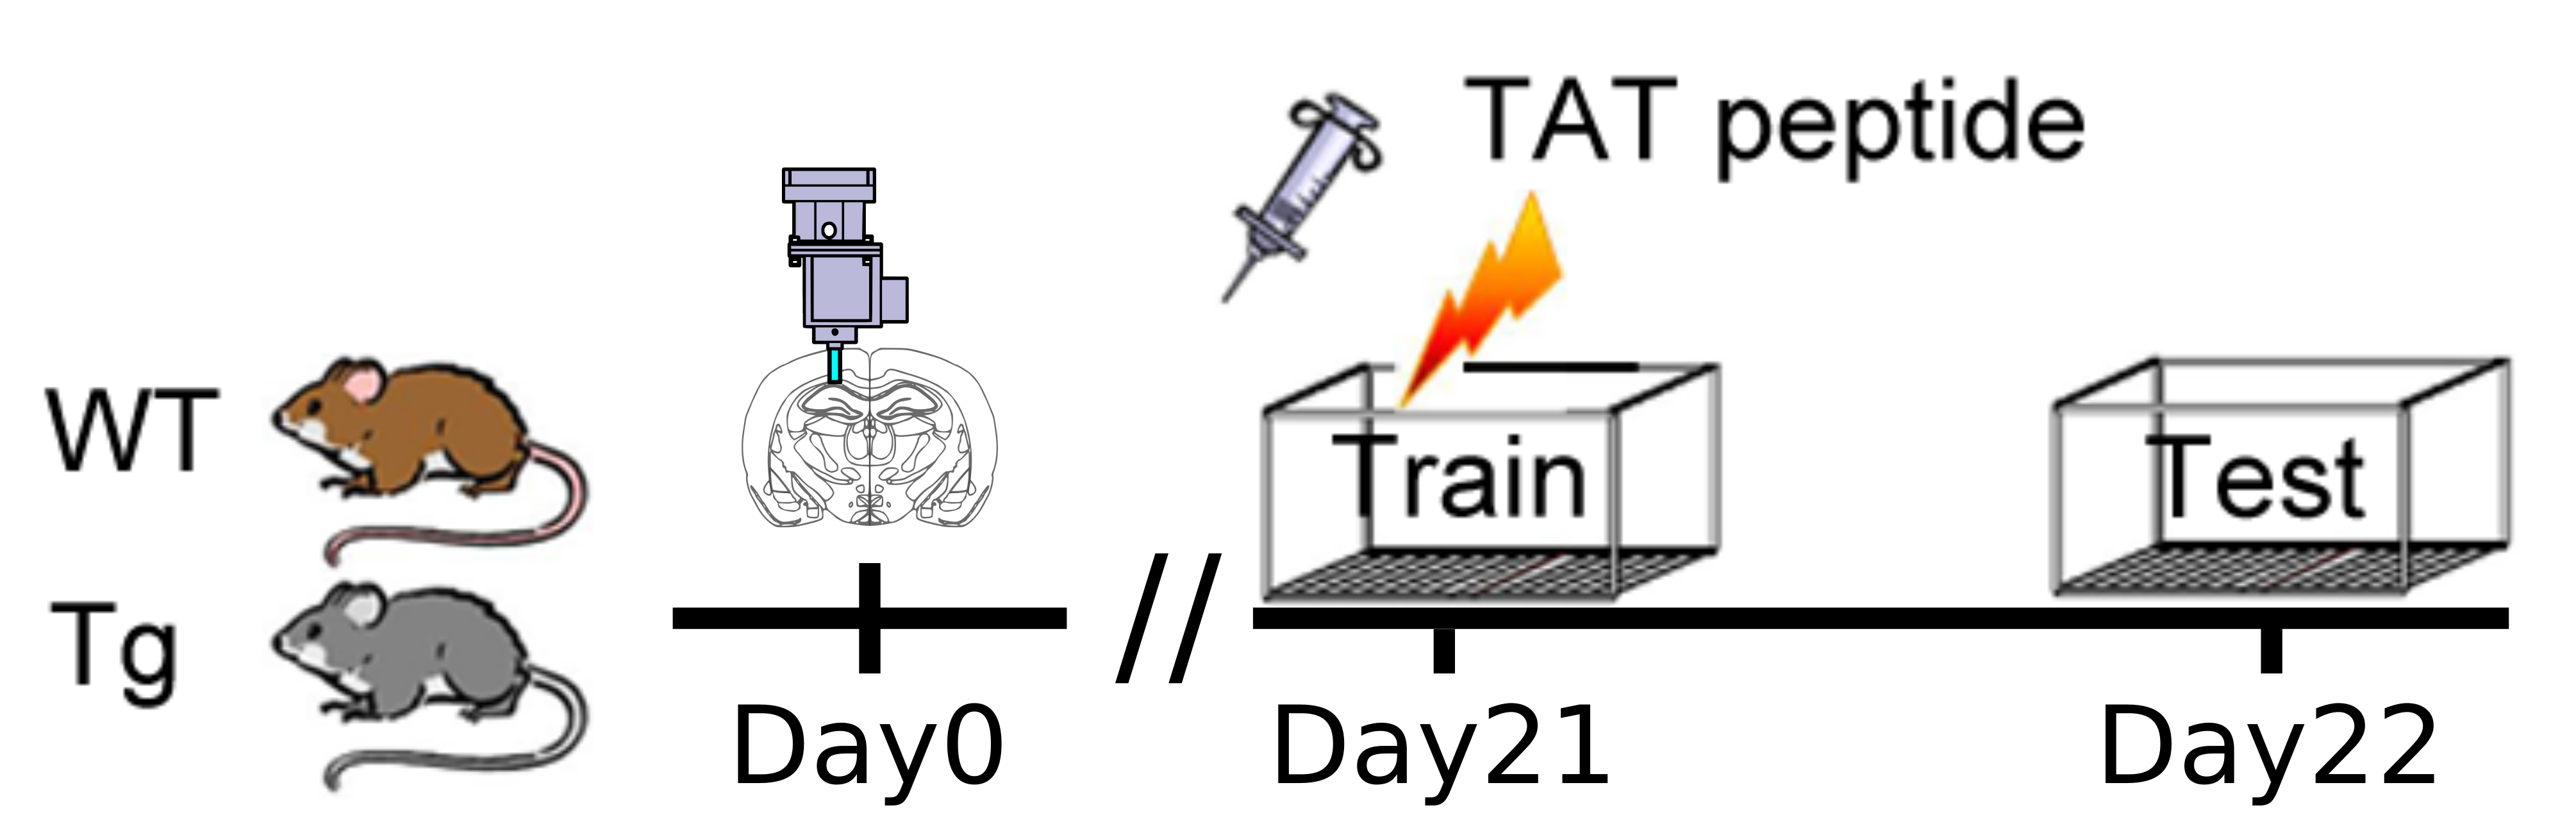
\includegraphics[width=\textwidth]{paradigm.png}
    \caption{Experimental paradigm. Adult \gls{wt} and \gls{tg} animals (with gCaMP6f expression) were implanted with a mini-microscope baseplate targeting CA1 hippocampus on day 0. The cells were visible three weeks later. Animals received \tglu peptide (i.p.) \SI{1}{\hour} before contextual fear conditioning. Animals were tested \SI{24}{\hour} later for freezing behaviour. Calcium activity were recorded for both training and testing session. \label{f.ad.paradigm}}
\end{figure}

\begin{figure}[h]
    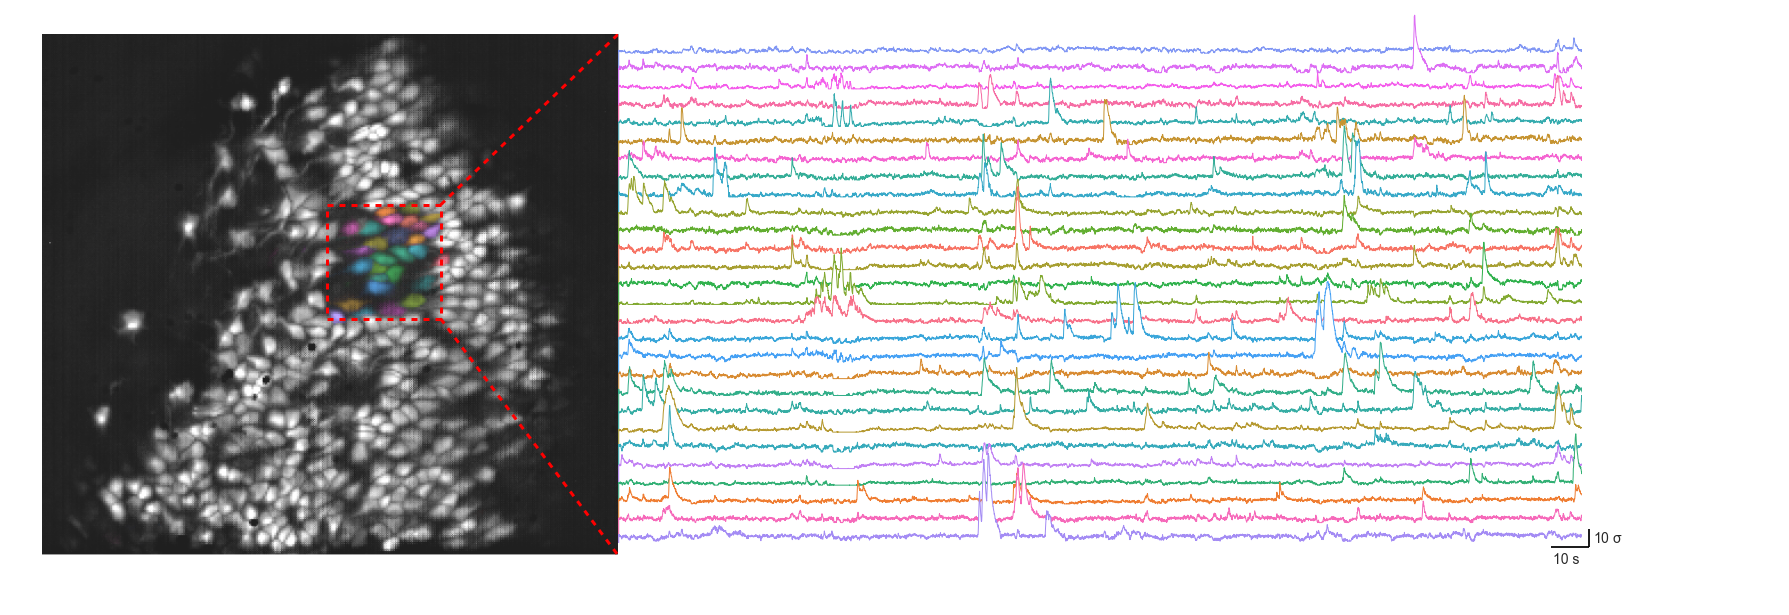
\includegraphics[width=\textwidth]{trace.png}
    \caption{Sample cell image and traces. Traces are random coloured and correspond to cells of the same colour. \label{f.ad.trace}}
\end{figure}

Figure~\ref{f.ad.freezing} shows the percent of freezing during testing. Two-way \gls{anova} has revealed significant main effect in genotype (F\tsb{1,27}=12.79, p=0.001) as well as a significant interaction between genotype and treatment (F\tsb{1,27}=5.45, p=0.027). Posthoc tests show that \gls{tg} animals have significant lower freezing (\gls{wt}-Veh vs \gls{tg}-Veh, T=4.21, p<0.001), and this effect is fully rescued by \tglu treatment (\gls{tg}-\tglu vs \gls{tg}-Veh, T=2.85, p=0.008; \gls{wt}-Veh vs \gls{tg}-\tglu, T=1.12, P=0.27). \tglu has no significant effect on \gls{wt} animals (\gls{wt}-Veh vs \gls{wt}-\tglu, T=0.355, p=0.72). This result is consistent with our hypothesis, Tg animals showed decreased freezing, and this was rescued by \tglu treatment. 

\todo{freezing}
\begin{figure}[h]
    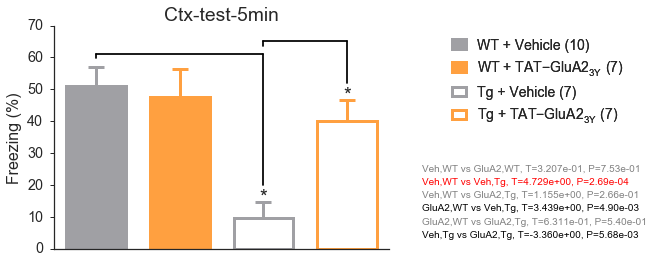
\includegraphics[width=\textwidth]{freezing.png}
    \caption{Percent of freezing during testing. \Gls{tg} animals have significant lower freezing, and \tglu treatment returns the freezing to wildtype level. \label{f.ad.freezing}}
\end{figure}



\subsection{\tglu rescues hyperactivity in \gls{tg} cells}

Figure~\ref{f.ad.acttrain} shows average cell activity during training session before footshock is delivered. During training, two-way \gls{anova} reveals significant major effects of genotype (F\tsb{1,3033}=6.2, p=0.01) and treatment (F\tsb{1,3033}=5.1, p=0.02) as well as a significant interaction between genotype and treament (F\tsb{1,3033}=7.7, p=0.006). Posthoc tests shows that \gls{tg}-Veh has significantly higher cell activity (WT-Veh vs Tg-Veh, T=-3.72, p<0.001), and \tglu treatment is able to restore average cell activity to \gls{wt} level. (Tg-\tglu vs Tg-Veh, T=-3.58, p<0.001; WT-Veh vs Tg-\tglu, T=0.14, p=0.89). \tglu does not have any effect on \gls{wt} animals (WT-Veh vs WT-\tglu, T=-0.137, p=0.89) This result is consistent with previous reports in the literature \citep{verret12}, showing cells in Tg animals have increase overall cell activity. Interestingly, while \tglu treatment restores the the mean cell activity during training, the distribution of cell activity is significantly different from \gls{wt} (WT-Veh vs Tg-\tglu, K=0.16, P<0.001). As is shown in the cumulative distribution plot, Tg-\tglu still have a over-proportion of highly active cells. 
\todo{Discuss: \tglu is not able to rescue cells with very high activity}

Similar effect were found during testing (Figure~\ref{f.ad.acttest}). Two-way \gls{anova} revealled significant major effect of genotype (F\tsb{1,3029}=32.7, p<0.001) and treatment (F\tsb{1,3029}=27.4, p<0.001), as well as their interaction (F\tsb{1,3029}=78.4, p<0.001). Post-hoc tests show significant increase of cell activity in Tg-Veh group (WT-Veh vs Tg-Veh, T=-10.1, p<0.001), and this effect is corrected by \tglu treament (WT-Veh vs Tg-\tglu, T=0.73, p=0.47; Tg-\tglu vs Tg-Veh, T=-9.97, p<0.001). There is also a trend of increase in cell activity after \tglu treatment in \gls{wt} group, however the p-value is close to threshold after correction of multiple comparison (WT-Veh vs WT-\tglu, T=-2.53, p=0.012, threshold = 0.013). Interestingly during testing, \tglu is able to fully rescue the hyper-activity in \gls{tg} group (\gls{kstest}: Veh-WT vs Tg-\tglu, K=0.06, p=0.07; Tg-Veh vs Tg-\tglu, K=2.29, p<0.001). These results suggest that the rescuing effect of \tglu in \gls{tg} animals is slow and long-lasting.

\begin{figure}[h]
    \begin{subfigure}[h]{\textwidth}
        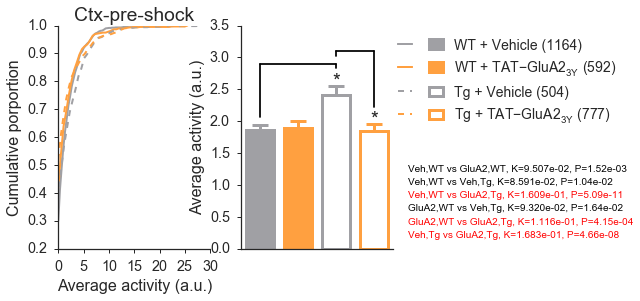
\includegraphics[width=\textwidth]{activity_train.png}
        \caption{\label{f.ad.acttrain}}
    \end{subfigure}
    \begin{subfigure}[h]{\textwidth}
        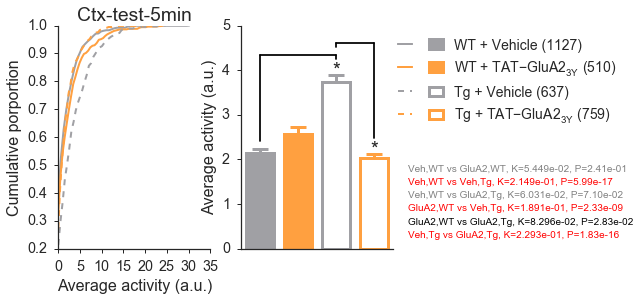
\includegraphics[width=\textwidth]{activity_test.png}
        \caption{\label{f.ad.acttest}}
    \end{subfigure}
    \caption{Distribution and mean of average cell activity during \subref{f.ad.acttrain} training and \subref{f.ad.acttest} testing. Cells in the Tg animals are significantly more active, and this is rescued by \tglu treatment. \label{f.ad.activity}}
\end{figure}

\subsection{\tglu rescues freezing encoding deficit in \gls{tg} cells}

We then investigated that how \gls{wt} and \gls{tg} cells encodes freezing. First we looked at cells individually, and calculated the mutual information between cell firing and freezing \citep{skaggs93}. This measurement reflects how much prediction power a cell has for freezing in a period of time. The group differences in freezing information is then compared using two-way \gls{anova}. There is significant main effect in both genotype (F\tsb{1,4380}=114.8, p<0.001) and treatment (F\tsb{1,4380}=7.3, p=0.007), and a significant interaction between the two factors (F\tsb{1,4380}=33.8, p<0.001). Posthoc tests show Tg-Veh group has significantly less freezing information (WT-Veh vs Tg-Veh, T=11.8, p<0.001), and this deficit is partially rescued by \tglu treatment (Tg-\tglu vs Tg-Veh, T=6.05, p<0.001), as there is a trend that Tg-\tglu group has less freezing information than WT-Veh group (WT-Veh vs Tg-\tglu, T=2.12, p=0.03, threshold=0.0125; Figure~\ref{f.ad.freeze_info}). This result suggests in the \gls{tg} group, the cell activity in hippocampus \gls{ca1} does not predict the animal's behaviour well, however this is improved with \tglu treatment but not fully rescued. 
\begin{figure}[h]
    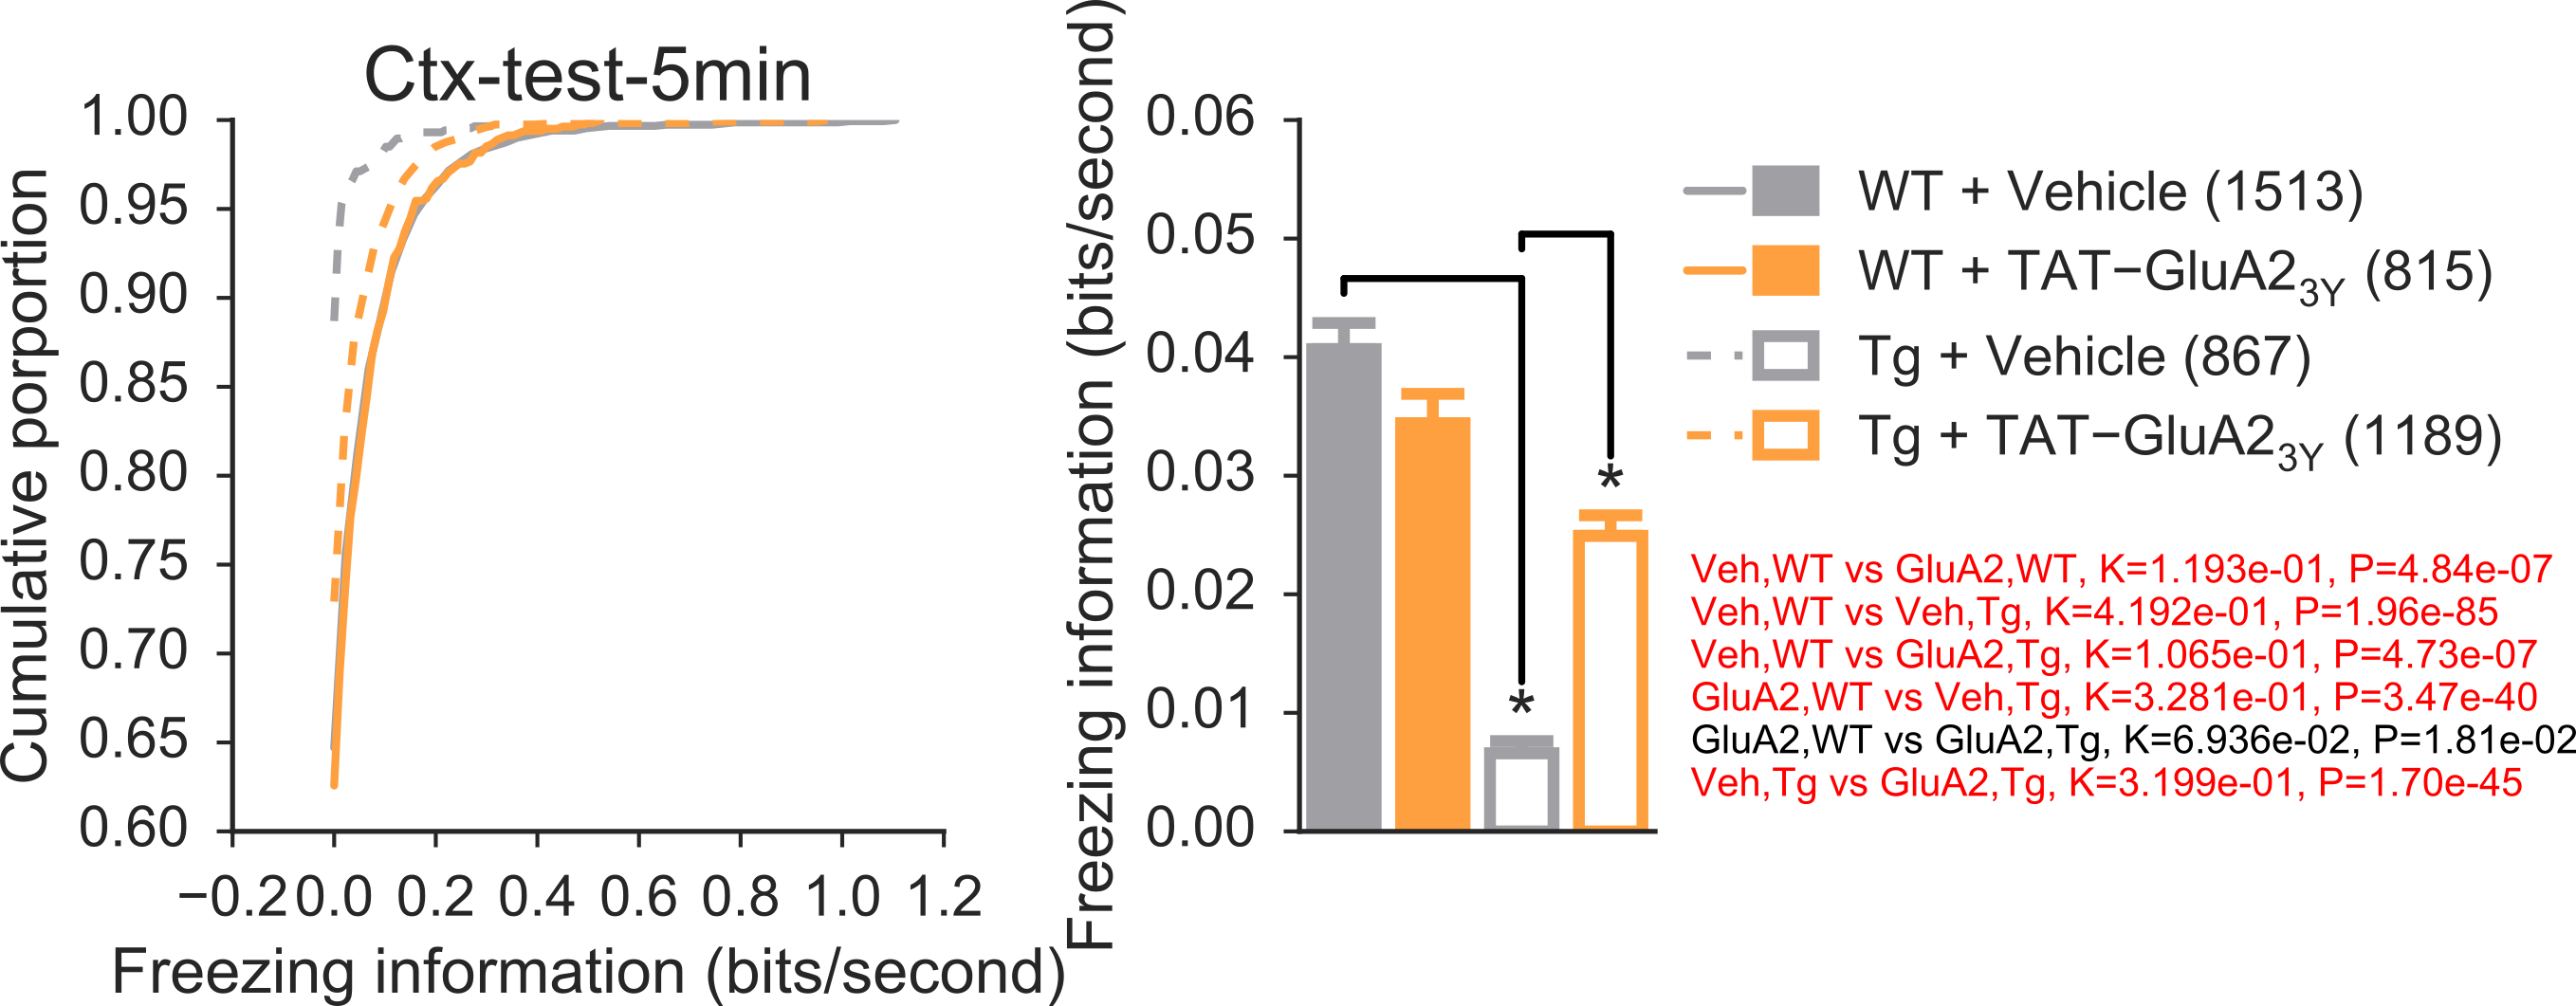
\includegraphics[width=\textwidth]{freeze_info.png}
    \caption{Freezing information during testing. This measurement represent how much information a cell have in a period of time about whether the animal is freezing. Cells in \gls{tg} animals encode significantly less freezing than the \gls{wt} groups, and \tglu treatment can only partially rescue the effect. \label{f.ad.freeze_info}}
\end{figure}
    

Then using machine learning methods, we investigated how freezing is encoded at a network level by training general classifiers to predict animals' behaviour from recorded cell activity. Both approach suggest that Tg animals have consistent worse freezing encoding both at a cellular level but also at a network level. 

While all the measurements we have performed considers each cell individually, are the cells independent of each other, or is part of the information encoded in the coordination between them? To answer this question, we have build two classifiers: a \gls{nbc} which models the cells independent of each other, and a \gls{gsvm}, which also uses the dependency between cells for prediction. The result is shown in Figure~\ref{f.ad.classifier}. 

A three-way \gls{anova} of genotype * treatment * classifier was carried out. There are significant main effect of genotype (F\tsb{1,50}=15.6, p<0.001), treatment (F\tsb{1,50}=5.5, p=0.02) and classifier (F\tsb{1,50}=9.0, p=0.004). There is also a significant interaction between genotype and treatment (F\tsb{1,50}=14.2, p<0.001), and no significant interactions involving classifier factor. Since the classifier factor only have a significant major effect, for the posthoc tests we used F-test to only compare different levels of genotype and treatment. F1 score of Tg-Veh is significantly less than WT-Veh (F\tsb{2,50}=16.4, p<0.001), and this effect is rescued by \tglu treatment (Tg-\tglu vs Tg-Veh, F\tsb{2,50}=9.7, p<0.001). There is no significant difference between WT-Veh and Tg-\tglu (F\tsb{2,50}=0.63, p=0.54), and \tglu treatment has no significant effect on \gls{wt} group (WT-Veh vs WT-\tglu, F\tsb{2,50}=0.20, p=0.81).  

These results show \gls{gsvm} significantly outperforms the \gls{nbc} classifier across all groups, suggesting that the network encodes more information than the cells individually. Moreover, both classifiers perform significantly worse in the \gls{tg} group, further supports our hypothesis that \gls{tg} animals have inferior fear memory encoding. Moreover, this deficit is fully rescued by \tglu treatment.

\begin{figure}[h]
    \begin{subfigure}[h]{\textwidth}
        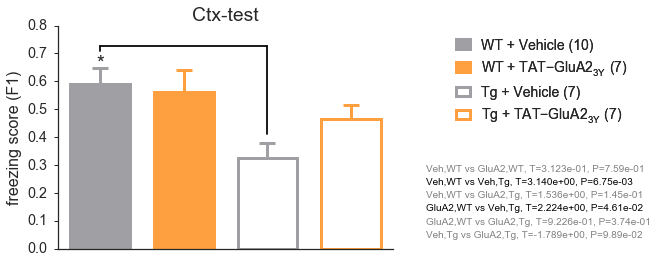
\includegraphics[width=\textwidth]{nb.png}
        \caption{\label{f.ad.nb}}
    \end{subfigure}
    \begin{subfigure}[h]{\textwidth}
        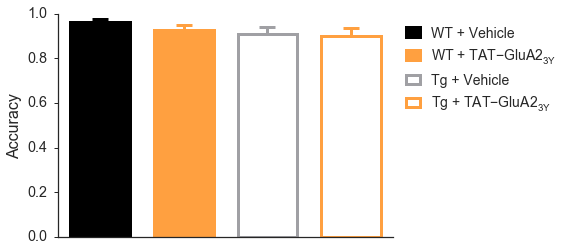
\includegraphics[width=\textwidth]{svm.png}
        \caption{\label{f.ad.svm}}
    \end{subfigure}
    \caption{Performance of \subref{f.ad.nb} \gls{nbc} and \subref{f.ad.svm} \gls{gsvm} in predicting freezing from cell activity. Results are measured as F1 score. Both classifiers showed inferior performance in \gls{tg} group, further supports the hypothesis that \gls{tg} animals have sub-optimal freezing encoding. Interestingly, since \gls{nbc} assumes the cells are independent and \gls{gsvm} is more general, the performance difference between the two suggest a portion of freezing information is encoded in the coordination between the activity of the cells. \label{f.ad.classifier}}
\end{figure}




\subsection{Difference of encoding in \gls{tg} animals is not a result of animal's behaviour}

However, given that the Tg animals also show behavioural difference, we then try to answer the question: is the difference in neural coding inherit of the Alzheimer animal, or a result of the different behaviour? Given that CA1 cells are known to represent place, we have calculated the freezing information marginalized over all animal positions, therefore eliminating it's effect in the calculation of freezing information. Two-way \gls{anova} shows significant main effects in genotype (F\tsb{1,4380}=112.8, p<0.001) and treatment (F\tsb{1,4380}=30.4, p<0.001), as well as significant interaction between the two factors (F\tsb{1,4380}=48.6, p<0.001). Posthoc tests show that Tg-Veh has significant lower freezing information with position controlled (WT-Veh vs Tg-Veh, T=12.5, p<0.001), and partially rescued by \tglu (Tg-\tglu vs Tg-Veh, t=8.85, p<0.001; WT-Veh vs Tg-\tglu, t=3.56, p<0.001). The result is similar and shown in Figure~\ref{f.ad.freeze_ctrl}.  
\begin{figure}[h]
    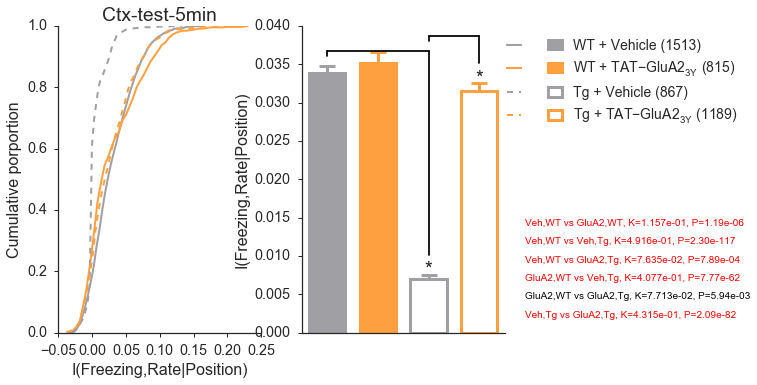
\includegraphics[width=\textwidth]{freeze_position.png}
    \caption{Freezing information conditioned on animal's position. This measurement removes the effect of position from freezing information measurement. This result is similar to Figure~\ref{f.ad.freeze_info}. This suggest that the position of the animal is not a confounding factor for freezing information measurement. \label{f.ad.freeze_ctrl}}
\end{figure}


An additional potential confound comes from the animal's behaviour. Within \gls{wt} animals, there is a significant correlation between freezing information and freezing \todo{stats and figure}. Given that \gls{tg} animals do not freeze well during testing, we ask is the encoding deficit found in \gls{tg} animals explained by the correlation of freezing and encoding? To investigate this question, we added freezing as a covariate into the two-way \gls{anova} model for position-controlled freezing information. The resulting model shows while percent of freezing is a significant confound in measuring freezing information (F\tsb{1,4379}=42.0, p<0.001), there is still significant major effect of genotype (F\tsb{1,4379}=34.0, p<0.001) and treatment (F\tsb{1,4379}=6.7, p=0.009), as well as a significant interaction between the two factors (F\tsb{1,4379}=5.6, p=0.017). Similarly to Figure~\ref{f.ad.freeze_ctrl}, Posthoc tests have found a significant decrease of freezing information in Tg-Veh with freezing level controlled (WT-Veh vs Tg-Veh, t=5.46, p<0.001), as well as a partial rescue by \tglu treatment (Tg-\tglu vs Tg-Veh, t=3.45, p=0.001; WT-Veh vs Tg-\tglu, t=2.93, p=0.003). And again, no effect of \tglu on \gls{wt} animals (WT-Veh vs WT-\tglu, t=-0.30, p=0.75). These results suggest that while freezing information is correlated with percent of freezing, \gls{tg} animals have additional deficit in encoding freezing, and this deficit is partially rescued by \tglu treatment. 

\begin{comment}
In addition, we also checked whether the freezing information coding is a result of different freezing or uneven spatial coverage of the behavioural chamber, which are represented by freezing entropy and spatial entropy respectively. To check these two factors, we have pooled the groups with similar behaviour (\gls{wt}, \gls{wt}-\tglu, \gls{tg}-\tglu), and correlated percent freezing, freezing entropy, total distance and spatial entropy against freezing information within the pooled groups. If the behavioural measurement have no influence in the freezing information, we would expect no correlation. Indeed, that is what we have found in Figure~\ref{f.ad.corrs}. These control measurements have shown that the reduction of freezing encoding in the Tg animals is not affected by the difference in the animals' behaviour.
\begin{figure}[h]
    \begin{subfigure}[t]{.5\textwidth}
        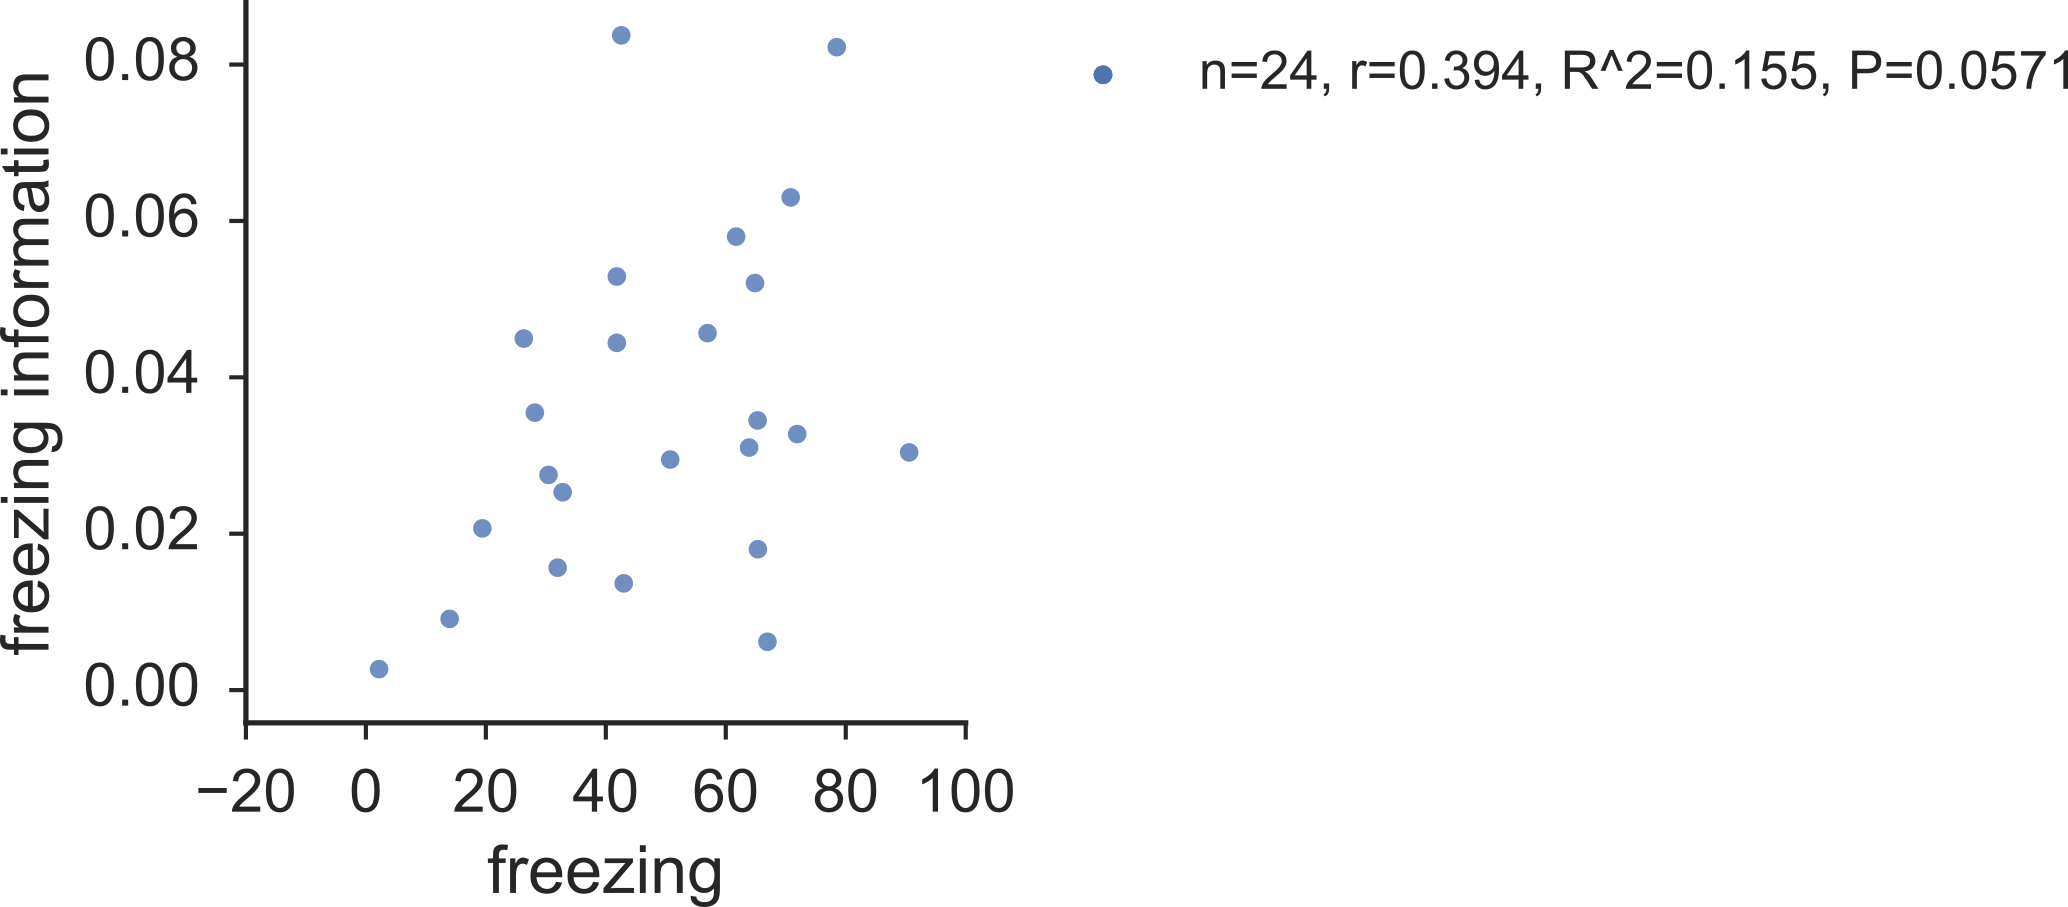
\includegraphics[width=\textwidth]{corr1.png}
        \caption{}
    \end{subfigure}
    \begin{subfigure}[t]{.5\textwidth}
        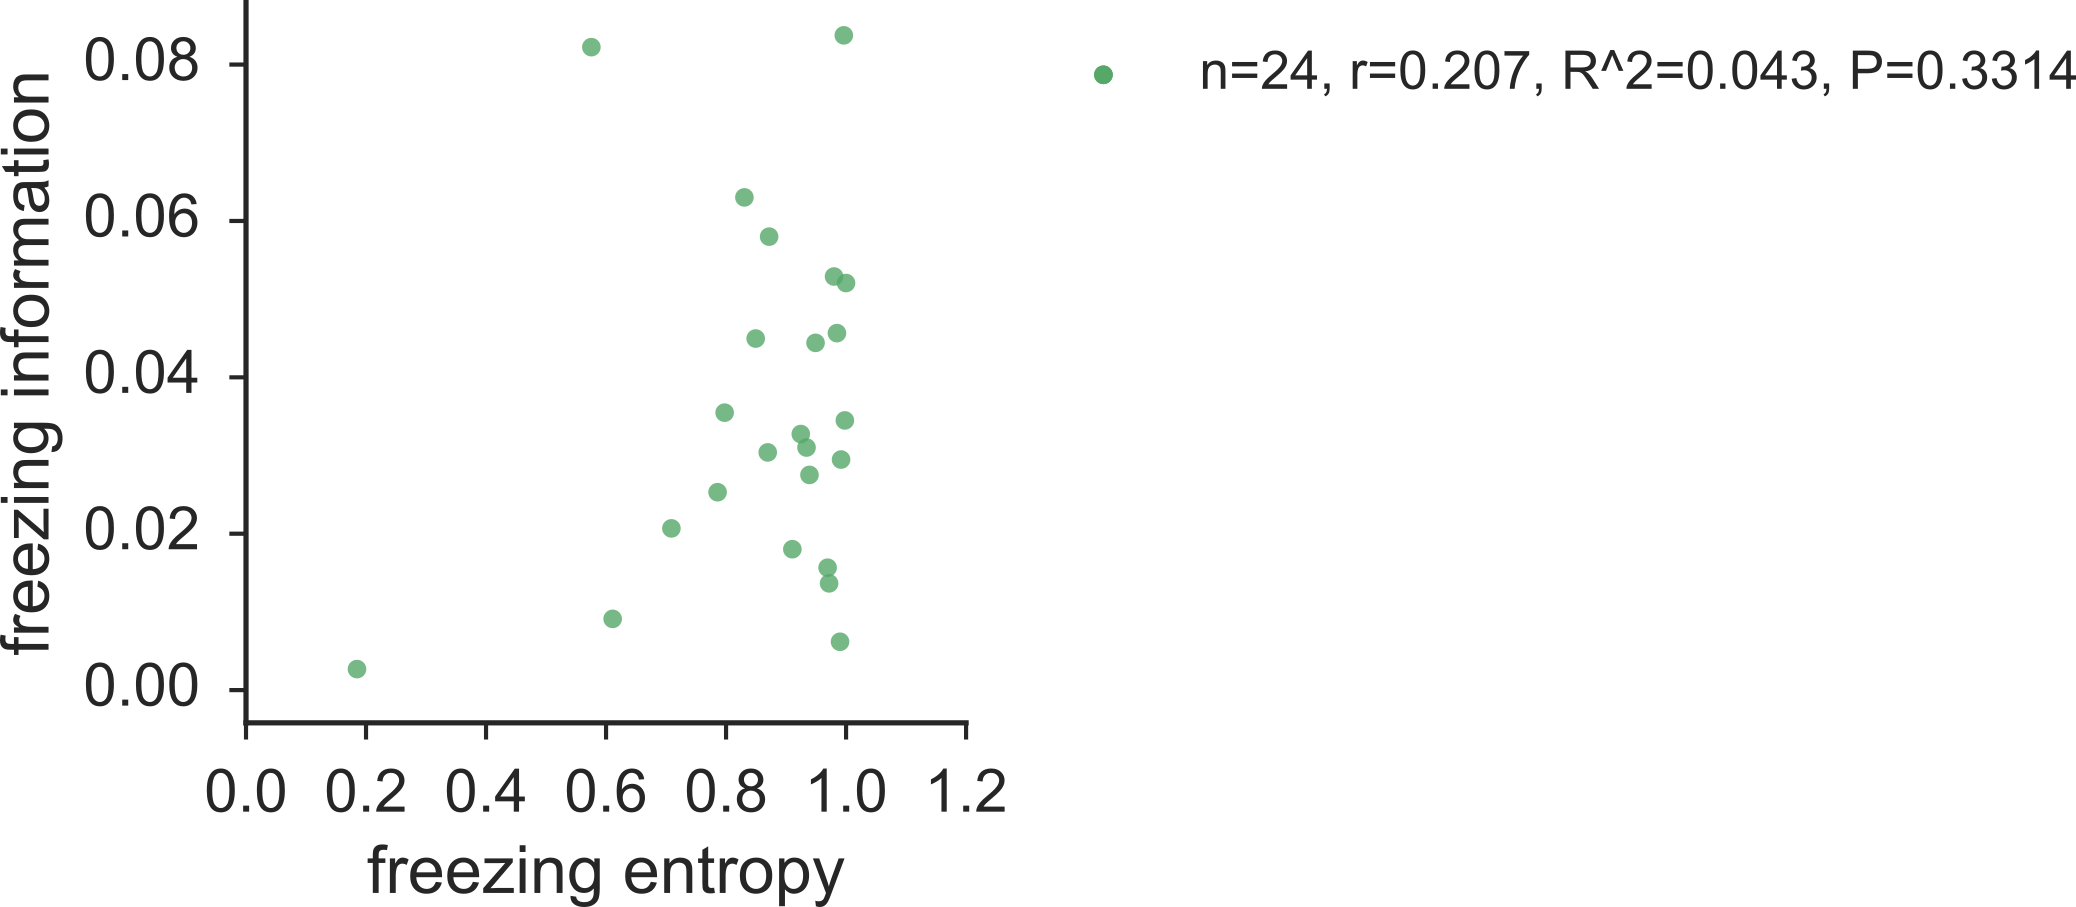
\includegraphics[width=\textwidth]{corr2.png}
        \caption{}
    \end{subfigure}
    \begin{subfigure}[t]{.5\textwidth}
        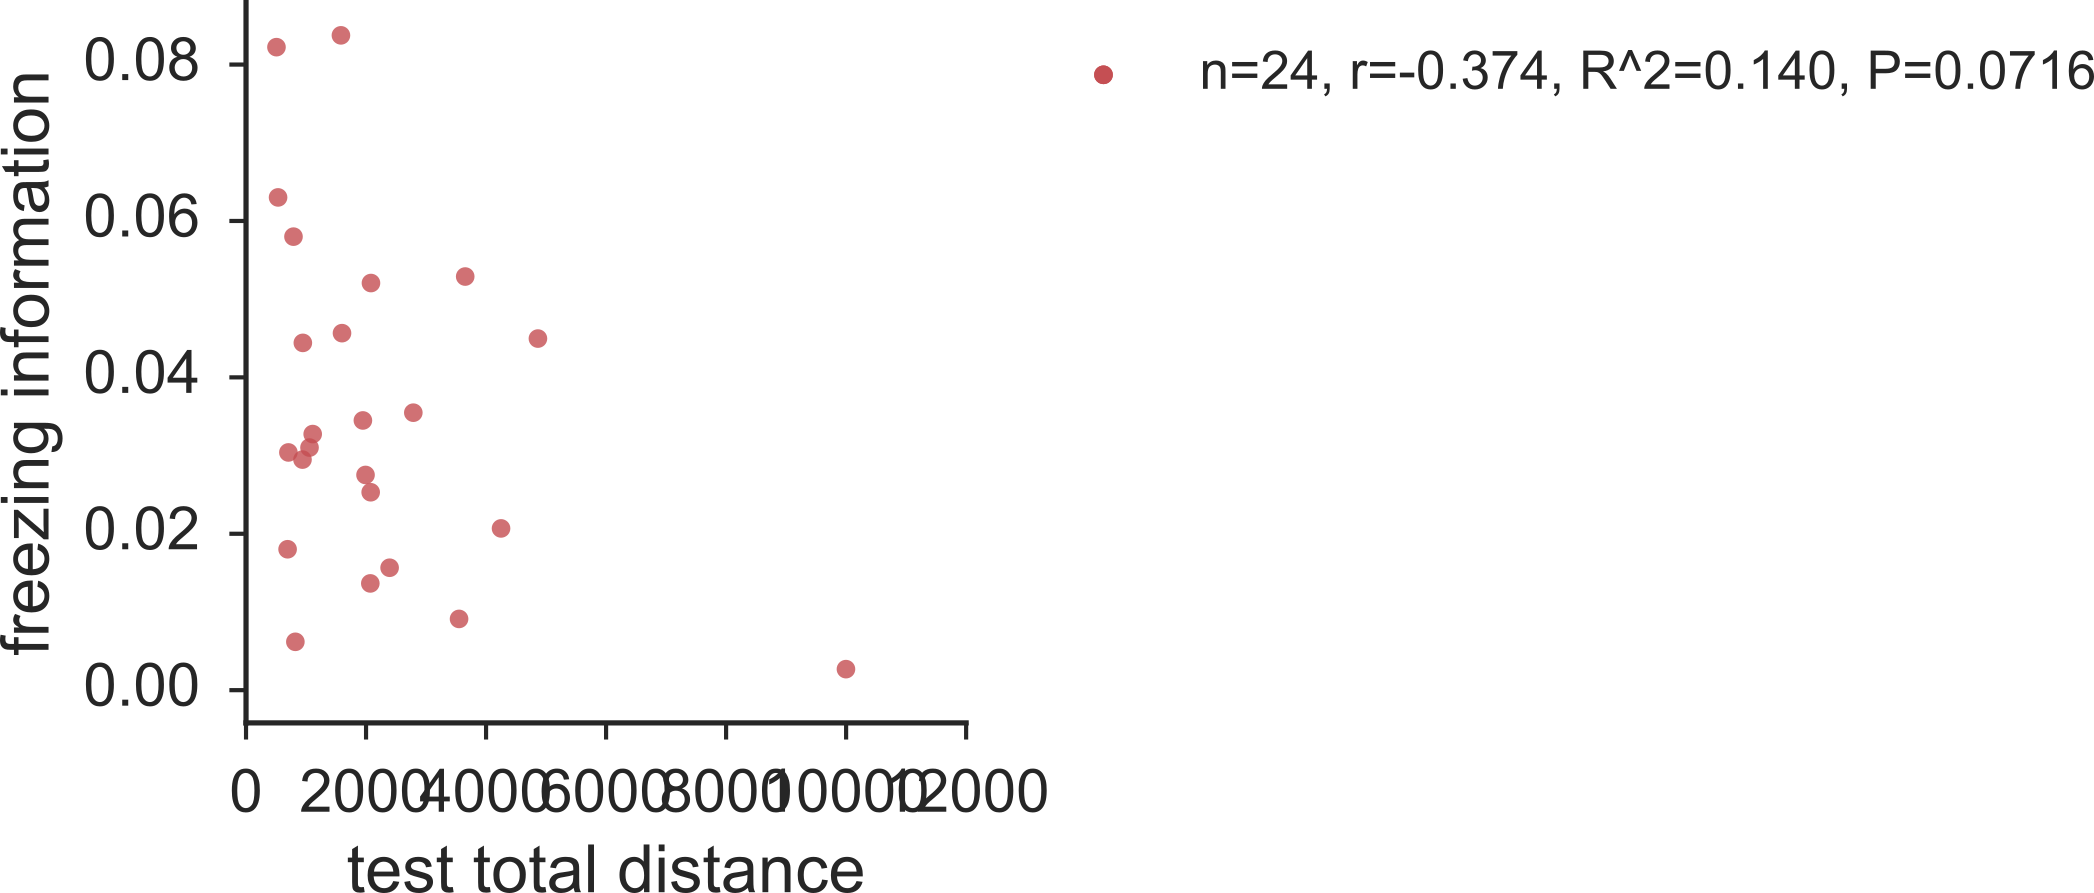
\includegraphics[width=\textwidth]{corr3.png}
        \caption{}
    \end{subfigure}
    \begin{subfigure}[t]{.5\textwidth}
        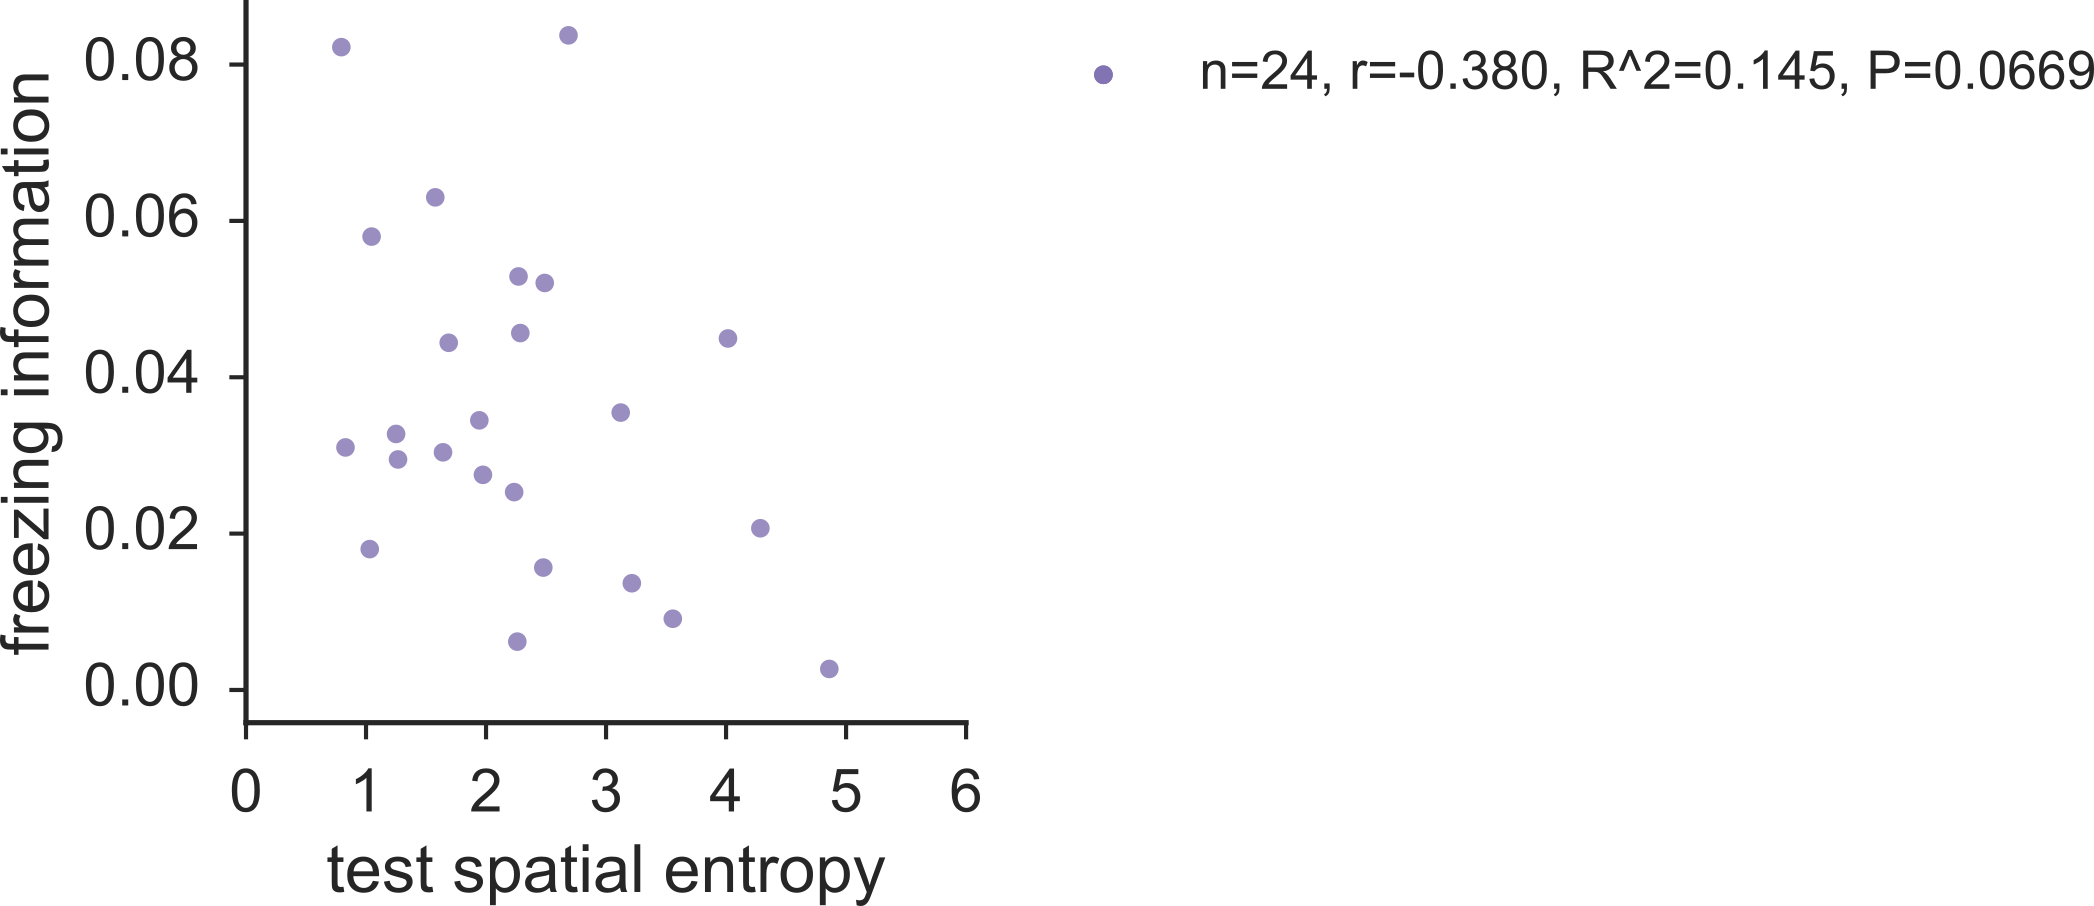
\includegraphics[width=\textwidth]{corr4.png}
        \caption{}
    \end{subfigure}
    \caption{Scatter plots of varies behaviour measurement against freezing information, in pooled \gls{wt}, \gls{wt}-\glu and \gls{tg}-\glu. Given there is no group difference between the three groups, if any of the behaviour factor is confounding, the it will contribute to within-group difference and correlate with freezing information. We have found no significant correlations. However the near significance of percent freezing and spatial entropy correlations will need further investigation. \label{f.ad.corrs}}
\end{figure}
\end{comment}


\subsection{\tglu rescues recall by decreasing activity}

The next question we investigated is, if the cells are encoding freezing, how do they encode? In figure~\ref{f.ad.ch_activity} we selected all the cells that have more than 0.01 bits/second (which amounts to ~40\% in the normal groups and 10\% of the cells in the \gls{tg} group), and plotted the difference of average activity when the animal is freezing and not freezing. Interestingly, majority of the cells encode freezing by decreasing their activity. This can also be seen representatively in the sample trace (Figure~\ref{f.ad.sample_trace}).
\begin{figure}[h]
    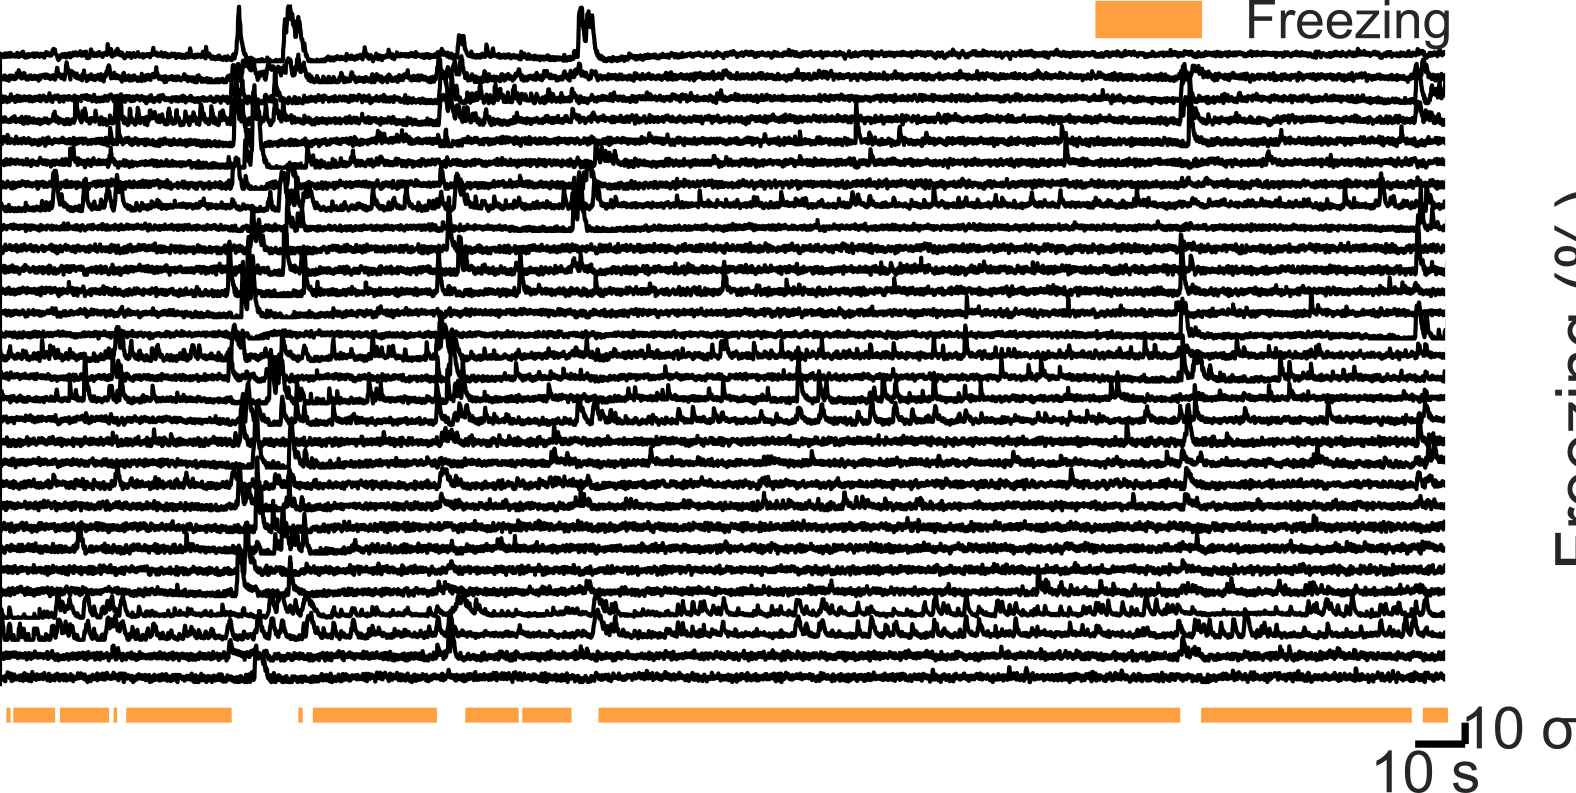
\includegraphics[width=\textwidth]{sample_trace.png}
    \caption{Sample traces from cells with highest freezing information in an animal. It appears that cells encode freezing by decreasing their activity. \label{f.ad.sample_trace}}
\end{figure}
\begin{figure}[h]
    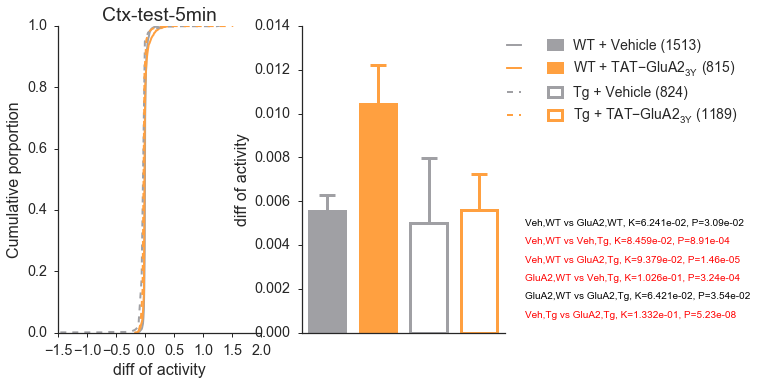
\includegraphics[width=\textwidth]{ch_activity.png}
    \caption{Distribution and mean of activity difference between freezing and none-freezing, in cell with freezing information more than 0.01. This confirms the intuition from Figure~\ref{f.ad.sample_trace} that most of the cells encode freezing by decreasing activity. \label{f.ad.ch_activity}}
\end{figure}

Given the cells tend to have decreased activity during freezing, we also examined the average cell activity when the animal is freezing, and activity when the animal is not (Figure~\ref{f.ad.activity_freezing}). Two-way \gls{anova} on the average activity when animals are freezing shows significant main effect in genotype (F\tsb{1,3034}=6.9, p=0.008) and treatment (F\tsb{1,3034}=18.7, p<0.001). The interaction between them is not significant (F\tsb{1,3034}=-0.03, p=0.97). \Gls{tg} animals show significantly increased activity during freezing, and \tglu treatment has a significant inhibitory effect on cell activity. \todo{discuss about highly active cells in the cumulative distribution plot}

Two-way \gls{anova} revealed a significant effect of treatment (F\tsb{1,3029}=12.3, p<0.001) and a significant genotype $\times$ treatment interaction (F\tsb{1,3029}=13.6, p<0.001). \tglu treatment only significantly decreased activity in the \gls{tg} animals (Tg-\glu vs Tg-Veh, T=-5.4, p<0.001). These results suggest the \tglu{} may rescue the \gls{tg} phenotype by globally decrease background cell activity.
\begin{figure}[h]
    \begin{subfigure}[h]{\textwidth}
        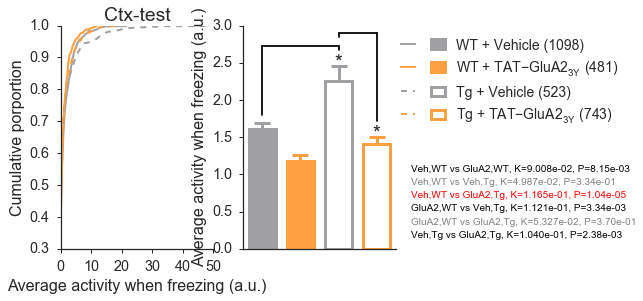
\includegraphics[width=\textwidth]{activity_freezing.png}
        \caption{\label{f.ad.actf}}
    \end{subfigure}
    \begin{subfigure}[h]{\textwidth}
        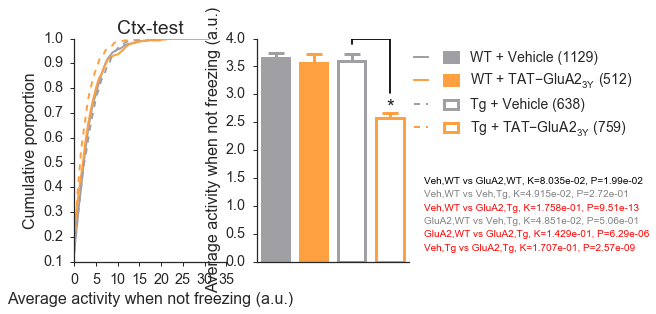
\includegraphics[width=\textwidth]{activity_moving.png}
        \caption{\label{f.ad.actnf}}
    \end{subfigure}
    \caption{Average cell activity during \subref{f.ad.actf} freezing and \subref{f.ad.actnf} not freezing. Cells in \gls{tg} animals have significantly higher activity during freezing, suggesting a sub-optimal encoding of freezing. Interestingly, \tglu also showed a decreased activity when the animal is not freezing, suggesting that the effect of \tglu maybe a global decrease of cell activity. \label{f.ad.activity_freezing}}
\end{figure}



\subsection{\Gls{tg} animals can initiate freezing}
We then investigated whether the deficits in \gls{tg} mice is due to less freezing initiation or freezing maintanence. Figure~\ref{f.ad.freezing_profile} summarizes the number and length of freezing periods in each group. There is no significant difference between groups in the number of freezing periods (Figure~\ref{f.ad.freezing_freq}, omnibus F\tsb{3,27}=0.84, p=0.48). On the length of freezing periods, there is significant main effect of genotype (F\tsb{1,27}=17.7, p<0.001), and a significant interaction between genotype and treatment (F\tsb{1,27}=6.5, p=0.01). Poshhoc tests shows Tg-Veh mice have significantly shorter freezing periods (WT-Veh vs Tg-Veh, T=4.75, p<0.001), and this deficit is fully rescued by \tglu treatment (Tg-\glu vs Tg-Veh, T=3.10, p=0.002; WT-Veh vs Tg-\glu, T=1.66, p=0.10). There is no effect of \tglu on \gls{wt} mice (T=0.22, p=0.83). 

\begin{figure}[h]
    \begin{subfigure}[h]{\textwidth}
        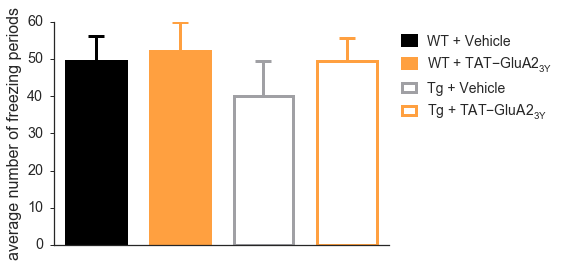
\includegraphics[width=\textwidth]{freezing_frequency.png}
        \caption{\label{f.ad.freezing_freq}}
    \end{subfigure}
    \begin{subfigure}[h]{\textwidth}
        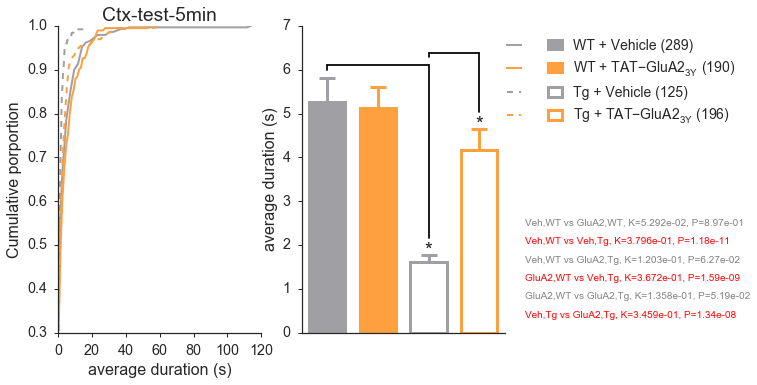
\includegraphics[width=\textwidth]{freezing_length.png}
        \caption{\label{f.ad.freezing_length}}
    \end{subfigure}
    \caption{Average number of freezing periods (\subref{f.ad.freezing_freq}) and length of freezing periods (\subref{f.ad.freezing_length}). \Gls{tg} mice freeze as often as \gls{wt} mice, but with less duration. This is rescued by \tglu treatment. \label{f.ad.freezing_profile}}
\end{figure}




\subsection{\Gls{tg} animals have deficits recall freezing memory}
\begin{figure}[h]
    \begin{subfigure}[h]{\textwidth}
        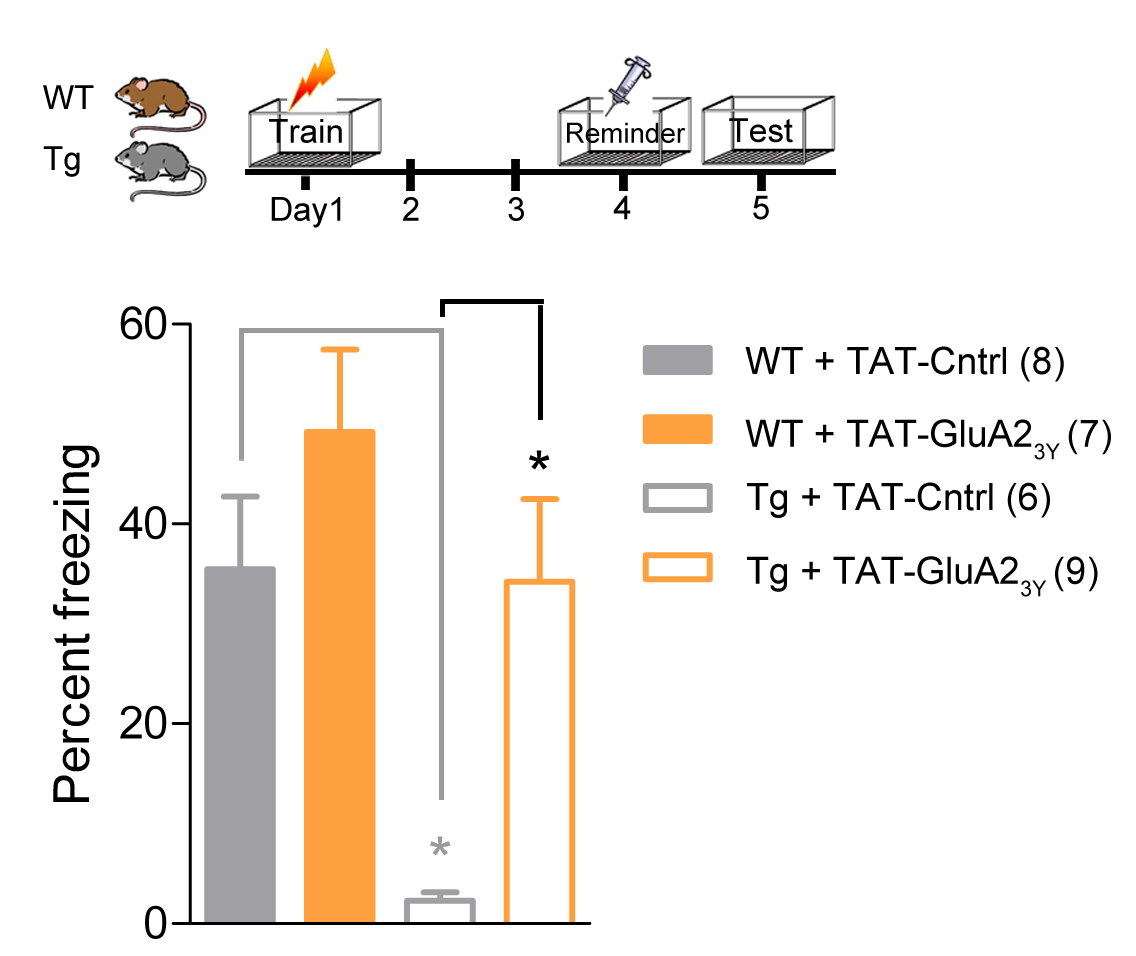
\includegraphics[width=\textwidth]{reminder1.png}
        \caption{\label{f.ad.actf}}
    \end{subfigure}
    \caption{ \label{f.ad.reminder1}}
\end{figure}

\section{Discussion}
\todo{Summary of result}
\todo{Hyperactivity}
\todo{Freezing encoding: not behavioural}
\todo{Direction of causation}
\todo{\tglu rescue - how?}
